% declare our document type
\documentclass[12pt]{article}

%%%%%%%% PACKAGES NEEDED FOR THIS DOCUMENT

% allow us to put pictures in the document
\usepackage{graphicx}
% this line lets us use larger fonts
\usepackage{extsizes}
% this allows us to create ''slides'' in the document
\usepackage[most]{tcolorbox}
% this line lets us caption images inside the ''slides''
% this is neccesary since the slide doesn't allow the use of
% \figure{} inside
\usepackage{caption}
\usepackage{courier}
\usepackage[hyphens]{url}
\usepackage[hidelinks]{hyperref}
\usepackage[margin=1in]{geometry}
\usepackage[utf8]{inputenc}
\usepackage[english]{babel}
\usepackage{cite}
\usepackage{listings}
\usepackage{textcomp}
\usepackage[
    type={CC},
    modifier={by-nc-sa},
    version={3.0},
]{doclicense}


\usepackage[T1]{fontenc}


%%%%%%%%%%% CUSTOM ENVIRONMENT SETUP

% declare a typesetting environment for code/emphasis
\newcommand{\code}[1]{\texttt{\bfseries#1}}
\newenvironment{codeblock}{\bfseries\texttt\bgroup}{\egroup\par}
% declare a large font environment for use in the ''slides''
\newcommand{\instruction}[1]{\Large{#1}}
\newenvironment{instructionblock}{\Large\bgroup}{\egroup}
% declare a ''slide'' text box for use in the document
% the slide is a numbered \section{}
\newtcolorbox[auto counter]{slide}[3][]{%
colback=brown!5!white,colframe=brown!80!gray,height from=4in to 9in,
title={\addcontentsline{toc}{section}{\thetcbcounter ~~ #2}\bf\Large\thetcbcounter ~ #2\hfill #3 \label{slide \thetcbcounter}\setcounter{section}{\thetcbcounter}}}
% declare a ''subslide'' text box for use in the document
% the subslide is a numbered \subsection{}
\newtcolorbox[auto counter,number within=section]{subslide}[3][]{%
colback=blue!5!white,colframe=blue!80!gray,height=3.72in,
title={\addcontentsline{toc}{subsection}{\thetcbcounter ~~ #2}\bf\Large\thetcbcounter ~ #2\hfill #3 \label{slide \thetcbcounter}}}
\renewcommand{\labelitemii}{$\circ$}
\lstset{basicstyle=\ttfamily,keywordstyle=\bfseries\color{blue!80!black},identifierstyle=\bfseries,stringstyle=\color{red},showstringspaces=false,commentstyle=\itshape\color{green!40!black},upquote=true}

% My Environments (keep these)
\newcommand{\ben}{\begin{enumerate}}
\newcommand{\een}{\end{enumerate}}
\newcommand{\bi}{\begin{itemize}}
\newcommand{\ei}{\end{itemize}}
\usepackage{titling}% for changelog
\newcounter{questionEnumerate}
\usepackage[anythingbreaks]{breakurl}%for breaking long url in references

%%%%%%%%% SET UP OUR TITLE PAGE

\begin{document}
\title{ Virtual Networks \\ \large and Secure Network Design}
\author{Hannah Pearson and Dillon Harris}
\date{August 12, 2017 \\ \hyperref[changelog]{Version 1.1}} %\today
\renewcommand{\abstractname}{Executive Summary}
\begin{titlepage}
\maketitle
\keepthetitle % for changelog
\pagenumbering{gobble}
\begin{center}

\includegraphics[scale=.5]{UofI}

\large{CS 539: Applied Security Concepts}

\vskip 40pt

\end{center}
\begin{abstract}
This tutorial will imparts knowledge regarding creation of virtual networks using VyOS. Specifically, we teach readers about the steps required to establish a network with three Ethernet interfaces, and which will have three zones associated with each interface. We hope that by the end of this tutorial, the readers will see a benefit of creating virtual networks through utilization of virtual routers such as VyOS or Pfsense.
\end{abstract}


\vfill
\begin{center}
	
\includegraphics[scale=0.5]{cc}
	\vskip 10pt
	This work is licensed under a \href{https://creativecommons.org/licenses/by/4.0/}{Creative Commons Attribution 4.0 International License}.
\end{center}

\end{titlepage}

%%%%%%%%%% TABLE OF CONTENTS

\pagebreak
\tableofcontents

%%%%%%%%%%%%%%%%%%%%%%%%%%%%%%%%%%%%%%%%%%%%%%%%%
%%%%%%    BEGINNING OF ACTUAL DOCUMENT
%%%%%%%%%%%%%%%%%%%%%%%%%%%%%%%%%%%%%%%%%%%%%%%%%

\pagebreak
\pagenumbering{arabic}
\setcounter{section}{1}
\begin{slide}{Prerequisites: Knowledge}{\hyperref[slide 2]{\textgreater}}
	\vskip 10 pt
	\begin{instructionblock}
Expected preparation:
    \begin{itemize}
    \item Understanding of the OSI model;
    \item Basic knowledge of IPv4 protocol;
    \item Experience with Linux systems and command line;
    \item Curiosity and motivation to learn.
    \end{itemize}
	\end{instructionblock}
\end{slide}

\pagebreak
\begin{slide}{Prerequisites: VM Infrastructure}{\hyperref[slide 1]{\textless}\hyperref[slide 3]{\textgreater}}
	\vskip 10 pt
	\begin{instructionblock}
Using a virtualization software, set up the following VMs; all in a unique port group.
    \begin{itemize}
    \item VyOS 1.1.7 with three network adapters;
    \item Windows 2012 R2 Server;
    \item Windows 10 Workstation;
    \item Ubuntu Web Server;
    \item Kali Workstation.
    \end{itemize}
	\end{instructionblock}
\end{slide}

Each group of VMs should be created on a distinct port group. In other words - ideally, each reader would have their own isolated network, which should be separated from other students' networks.


%----------------------------------------------------------------------------------------------------%





\pagebreak
\begin{slide}{Network Layout}{ \hyperref[slide 2]{\textless}\hyperref[slide 4]{\textgreater} }
	\vskip 5pt
	\begin{instructionblock}
		\begin{center}
			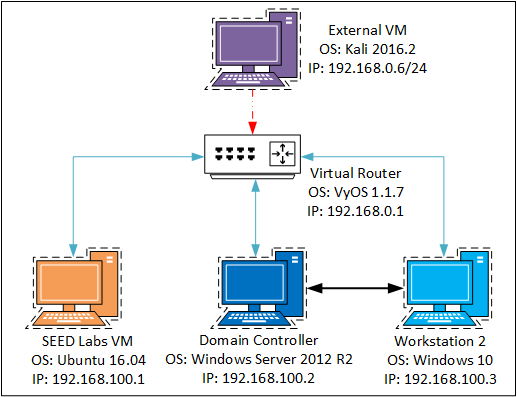
\includegraphics{NetworkDiagram.png}
		\end{center}
	\end{instructionblock}
\end{slide}


%----------------------------------------------------------------------------------------------------%



\pagebreak
\pagenumbering{arabic}
\setcounter{section}{1}
\begin{slide}{Router Overview}{\hyperref[slide 3]{\textless}\hyperref[slide 5]{\textgreater}}
	\vskip 10 pt
	\begin{instructionblock}
    Proper network configuration is the first line of defense.\\
    Open source routers for configuring small to mid-size networks:
    \begin{itemize}
    \item VyOS - Open source network OS.
    \item Pfsense - Open source firewall/router.
    \end{itemize}
    Both VyOS and pfSense are powerful and flexible enough to configure a secure network that accomodates a given company's unique requirements. 

	\end{instructionblock}
\end{slide}
\par Properly configuring a network is the first line of defense against malicious intruders and can be accomplished by configuring a router. Two commonly used open source routers for small to mid-size networks are VyOS, which is the open source version of Vyatta, and pfSense. VyOS offers only a command line, while pfSense features both a command line and a graphical interface. 


\pagebreak
\begin{slide}{VyOS Features}{\hyperref[slide 4]{\textless}\hyperref[slide 6]{\textgreater}}
	%\vskip 10 pt
	\begin{instructionblock}
    \begin{enumerate}
    \item VLANs;
    \item Static and Dynamic routing;
    \item Firewall;
    \item VPN;
    \item NAT;
    \item DHCP. 
    \end{enumerate}		
	\end{instructionblock}
\end{slide}
%\vfill
\begin{enumerate}
	\item VLANs - A virtual LAN (VLAN) is any broadcast domain that is partitioned and isolated in a computer network at the data link layer (OSI layer 2).
    \item Static/Dynamic Routing - BGP for IPv4 and IPv6.
    \item Firewall - Firewall rulesets for IPv4 and IPv6 traffic you can assign to interfaces, zone-based firewall, address/network/port groups for IPv4 firewalls.
    \item VPN - Site-to-site IPsec for IPv4 and IPv6, L2TP/IPsec server, PPTP server, OpenVPN for site-to-site and remote access.
    \item NAT - Source NAT, port forwards, one to one, one to many, and many to many translations.
    \item DHCP - DHCP and DHCPv6 server and relay.
\end{enumerate}

\pagebreak
\begin{slide}{Questions}{\hyperref[slide 5]{\textless}\hyperref[slide 7]{\textgreater}}
	%\vskip 10 pt
	\begin{instructionblock}
    \begin{enumerate}
    \item What is a reason you would want to setup VLANs in a network?
    \item What is the benefit of setting up a VPN?
    \item What is a DMZ and why would you want to use it?
    \item What does DHCP stand for?
    \end{enumerate}		
	\end{instructionblock}
\end{slide}
\begin{enumerate}
\item VLAN's allow a network manager to logically segment a LAN into different broadcast domains. Since this is a logical segmentation and not a physical one, workstations do not have to be physically located together.
\item A VPN (Virtual Private Network) is a way of adding an extra level of privacy to your online activity. VPNs encrypt your device’s internet connection, allowing you to surf the web privately.
\item The purpose of a DMZ is to add an additional layer of security to an organization's local area network (LAN); an external network node can access only what is exposed in the DMZ, while the rest of the organization's network is firewalled.
\item Dynamic Host Configuration Protocol
\end{enumerate}


\pagebreak
\begin{slide}{Network Routing}{\hyperref[slide 6]{\textless}\hyperref[slide 8]{\textgreater}}
	\vskip 10 pt
	\begin{instructionblock}
		\begin{enumerate}
		\item Process of selecting a path for network traffic;
        \item Packet forwarding;
        \item Routing tables.
		\end{enumerate}
	\end{instructionblock}
\end{slide}
\begin{enumerate}
\item Routing is the higher-level decision making that directs network packets from their source toward their destination through intermediate network nodes by specific packet forwarding mechanisms.
\item  Packet forwarding is the transit of logically addressed network packets from one network interface to another. Intermediate nodes are typically network hardware devices such as routers, bridges, gateways, firewalls, or switches.
\item The routing process usually directs forwarding on the basis of routing tables, which maintain a record of the routes to various network destinations.
\end{enumerate}


\pagebreak
\begin{slide}{Introduction to VyOS}{\hyperref[slide 7]{\textless}\hyperref[slide 9]{\textgreater}}
	\vskip 10 pt
	\begin{instructionblock}
		\begin{itemize}
        \item Linux-based network OS;
        \item Free and open source;
        \item Network routing, firewall, and VPN;
        \item Started in 2013 from GPL portions of Vyatta Core 6.6R1;
        \item Created after community edition of Vyatta was discontinued.
		\end{itemize}
	\end{instructionblock}
\end{slide}
\par VyOS is based on Debian GNU/Linux and is free and open source \cite{vyoswiki}. It was forked from parts of Vyatta, another very similar network operating system, which up until 2013 had a free community edition. When this was discontinued, VyOS was developed from Vyatta source liscenced under GPL \cite{vyoswiki}.


\pagebreak
\begin{slide}{VyOS Basics}{\hyperref[slide 8]{\textless}\hyperref[slide 10]{\textgreater}}
\begin{instructionblock}
\begin{itemize}
\item VyOS has two modes, configuration and operational;
\item Configuration (prompt ends in \texttt{\#}) for changing rules;
\item Operational (prompt ends in \texttt{\$}) for showing status;
\item Enter configuration mode by typing \texttt{conf};
\item Exit configuration mode by typing \texttt{exit};
\item Save changes: \texttt{commit \&\& save; exit}.
\end{itemize}
\end{instructionblock}
\end{slide}

\par There are two different types of users in VyOS, admin and operator \cite{vyoswiki}. The operator user can only use operational mode, meaning they can only view existing rules and monitor the network; Operator users cannot modify the configuration. Admin users, on the other hand, have full privileges and can change the network configuration \cite{vyoswiki}. 
\par In accordance with the principle of least privilege, a user should have the privileges they need to do their job and no greater. This means that ordinary day-to-day network monitoring can (and should) be done using an operator account. For setting up and configuring a network, like we are doing today, an administrator account is necessary. 

\pagebreak
\begin{slide}{Task 1: Replace Default User Account}{\hyperref[slide 9]{\textless}\hyperref[slide 11]{\textgreater}}
\begin{instructionblock}
Task 1: Create a new admin user. Log out and log back in using the new user. Remove the default VyOS user (vyos). 
\end{instructionblock}
\end{slide}

\noindent Users can be added using the following commands \cite{vyoswiki}:
\begin{lstlisting}
set system login user jsmith full-name "Johan Smith" 
set system login user jsmith authentication plaintext-password 
							password1 
set system login user jsmith level admin 
\end{lstlisting}
Existing users can be viewed in configuration mode using the command \cite{vyoswiki}:
\begin{lstlisting}
show system login
\end{lstlisting}
In operational mode, it is only possible to see a list of users and not the full contents of the configuration file, by using:
\begin{lstlisting}
show system login users
\end{lstlisting}
To delete a user, type the following in configuration mode:
\begin{lstlisting}
delete system login user [name of user to be deleted]
\end{lstlisting}
Be sure to commit changes before exiting.


\pagebreak
\begin{slide}{VyOS Basic Commands}{\hyperref[slide 10]{\textless}\hyperref[slide 12]{\textgreater}}
\begin{instructionblock}
\begin{itemize}
\item IP Configuration - vyos@vyos\$ show interfaces
\item Routing - vyos@vyos\$ show ip route
\item Show Configuration - vyos@vyos\$ show
\item Show log - vyos@vyos\$ monitor log, show log tail
\item Configure Interfaces - vyos@vyos\# set interfaces
\end{itemize}
\end{instructionblock}
\end{slide}
VyOS has the great feature of hitting tab for auto complete. This will come in handy for the tasks in this presentation. When in doubt hit tab and see the command options you can use.

\newpage
\begin{slide}{Introduction to Zones}{\hyperref[slide 11]{\textless}\hyperref[slide 13]{\textgreater}}
\begin{instructionblock}
\begin{itemize}
\item Useful for large or complex networks;
\item Usual non-zone based approach is to specify inbound/outbound rules per interface;
\item Zones can be used to combine multiple interfaces;
\item Firewall rules can be set for communication between zones;
\item Communication between zones is blocked by default.
\end{itemize}
\end{instructionblock}
\end{slide}
\par Once zones have been created, they can be used to design and implement firewall rules \cite{zonebasedfw}. For example:
\begin{lstlisting}
set zone-policy zone INSIDE from OUTSIDE firewall name INSIDE-OUT
\end{lstlisting}


\pagebreak
\begin{slide}{Discussion: Purpose and Application of Zones}{\hyperref[slide 12]{\textless}\hyperref[slide 14]{\textgreater}}
\begin{instructionblock}
\begin{itemize}
\item Why are zones useful? They seem like a pain...
\item Answer: Well. Consider the scenario described below, drawn today for your convenience on the whiteboard.
\item Discuss: How would you set up this network? What other scenarios can you envision in which zone-based firewalls might be of value?
\item How is the application of firewall rules to zones similar to the application of group policy to a domain? How is it different? Is this a helpful mental analogy?
\end{itemize}
\end{instructionblock}
\end{slide}

\par We don't have a large network set up, but you might imagine a scenario in which a large company wants to apply the principle of least privilege and limit access to specific resources to only those who need it. 

\par For example, your company's large software development team, which is distributed across three different network interfaces, has a server they use as a software repository and the marketing team, which uses two network interfaces, has a separate server they use for storing financial records.

\par Both groups have access to yet another the company's internal website and employee directory as well as the external public website located on one DMZ. Only the marketing group has access to a second external website, located on DMZ\_2, which is used by current clients of the software company.

\pagebreak
\begin{slide}{Questions}{\hyperref[slide 13]{\textless}\hyperref[slide 15]{\textgreater}}
\begin{instructionblock}
\begin{enumerate}
\item What is a LAN?
\item What is a WAN?
\item What are couple of differences between the two?
\end{enumerate}
\end{instructionblock}
\end{slide}
\begin{enumerate}
\item A LAN is a local area network, usually comprised of computers, printers, and etc in a local area like a building or office.
\item A WAN is a wide area network that is made up of multiple LANs.
\item A LAN will usually have a much higher bandwidth, then a WAN. People can setup their own LAN, but they don't usually setup WANs since a typical WAN connects LANs that could be 100's, or 1000's of miles apart.
\end{enumerate}

\pagebreak
\begin{slide}{Task 1: Network Design}{\hyperref[slide 14]{\textless}\hyperref[slide 16]{\textgreater}}
\begin{instructionblock}
Design a network topology that separates the following hosts and servers into appropriate logical zones using the VyOS 1.1.7 Router that has been provided:
\begin{itemize}
\item Domain Controller - Windows 2012 Server;
\item Workstation - Windows 10;
\item Web Server - Ubuntu 16.04 (DMZ);
\item Untrusted External Entity - Kali 2.0.
\end{itemize}
\end{instructionblock}
\end{slide}

\par This task is a preliminary task to the technical process of actually setting up the network and can be done on paper. Consider what machines need to be accessible to whom, and use this information to divide the virtual machines into logical zones.

\par In an actual network, this logical separation would be mapped to actual physical separation. For the purposes of this lab, it suffices to envision the physical separation while accepting that it is not practical to actually implement. 



\pagebreak
\begin{slide}{Challenge 1: Network Setup}{\hyperref[slide 15]{\textless}\hyperref[slide 17]{\textgreater}}
\begin{instructionblock}
Implement the zoned network you designed earlier using subnets.
\end{instructionblock}
\end{slide}

\begin{itemize}
\item Hint: there should be three subnets -- use the three ethernet interfaces on the VyOS router. (Google is your friend!)
\end{itemize}

\par Note that in our configuration, due to practical constraints, these ethernet interfaces all correspond to the same VLAN (specifically, in VMWare, the same port group). In an actual network, the zones should be physically separated at this level, so try to envision this separation in your mental model of the network. 


\pagebreak
\begin{slide}{NAT Background}{\hyperref[slide 16]{\textless}\hyperref[slide 18]{\textgreater}}
\begin{instructionblock}
Question 1: How many possible IPv4 addresses exist?
\\\\\\
Contrast this number with the estimated number of devices that will be connected to the Internet this year: \\20 billion \cite{ieeeiot}.
\\\\\\
How is this possible? How would you solve this problem? Anyone know how this problem was solved?
\end{instructionblock}
\end{slide}
See appendix for answer to Question 1.
\newline
\par One step to the solution was to abolish network classes (classes A, B, and C, representing networks containing 16,777,216 addresses, 65,536 addresses, and 256 addresses respectively) in favor of using more specific subnet masks, so networks that were too large for class C subnets but not large enough to use an entire class B subnet were able to free up IP addresses they did not need without an excessive strain on routers and routing tables which would otherwise have to manage mappings between multiple smaller class C networks \cite{arsipv4}.
\par The big breakthrough, though, was NAT. NAT, or Network Address Translation, enables one single IP address to represent an entire subnet. The following address ranges are specifically reserved for internal subnets: 10.0.0.0/8, 172.16.0.0/12, and 192.168.0.0/16 \cite{arsipv4}. Also, by convention, the router is assigned the address ending in .1, such as 192.168.0.1 or 10.0.0.1 for example.


\pagebreak
\begin{slide}{NAT Basics}{\hyperref[slide 17]{\textless}\hyperref[slide 19]{\textgreater}}
\begin{instructionblock}
\begin{itemize}
\item Two types of NAT;
\item Source NAT (sometimes simply referred to as NAT);
\item Source NAT bought time for IPv4 address problem;
\item Destination NAT (Port Forward);
\item Example use of port forwarding: setting up a minecraft server to use with friends on your home network.
\end{itemize}
\end{instructionblock}
\end{slide}
\par Source NAT (also known as Port Address Translation or NAT Overload) allows an entire subnet of machines to communicate with the internet from one IP address \cite{vyoswiki}. It was invented as a solution to the dwindling number of available IPv4 addresses in relation to the number of internet connected devices several decades ago \cite{arsipv4}. To set up a source NAT rule, the following information is required:
\begin{itemize}
\item Internal IP address to translate from;
\item Outgoing interface through which the address is to be translated;
\item External IP address to translate to.
\end{itemize}


\par Destination NAT, on the other hand, is used to direct \emph{external} traffic to a specific \emph{internal} host via a port behind a firewall.
Note that setting up a Destination NAT rule requires the following things \cite{vyoswiki}:
\begin{itemize}
\item Interface of incoming traffic;
\item Protocol and destination port;
\item Internal address to forward traffic to;
\end{itemize}



\pagebreak
\begin{slide}{Challenge 2: Source NAT Configuration}{\hyperref[slide 18]{\textless}\hyperref[slide 20]{\textgreater}}
\begin{instructionblock}
Challenge 1: Configure source NAT rules for both zones in your internal network.
\end{instructionblock}
\end{slide}
\par For this task you should map "internal IP addresses" (addresses of hosts belonging to the private zone subnet) to a the external facing gateway IP address, so that your boss, who is using the Windows 10 workstation, can access the internet. 

%\pagebreak
%\begin{slide}{Challenge 2: Destination NAT Configuration}{\hyperref[slide 11]{\textgreater}}
%\begin{instructionblock}
%Challenge 2: Configure a destination NAT rule to route traffic to your web server.
%\end{instructionblock}
%\end{slide}
%\par For this task you should map external traffic directed to port 80 (HTTP) to the Ubuntu web server in your DMZ. 

%There are two types of NAT: Source NAT and Destination NAT. The following are %commands for VyOS to setup our NAT rules for the network.

%\begin{enumerate}
%\item set nat source rule 10 outbound-interface eth0
%\item set nat source rule 10 source address 10.0.0.0/24
%\item set nat source rule 10 translation address masquerade
%\item set nat source rule 11 outbound-interface eth0
%\item set nat source rule 11 source address 10.0.1.0/24
%\item set nat source rule 11 translation address masquerade
%\end{enumerate}

\pagebreak
\begin{slide}{NAT Question}{\hyperref[slide 19]{\textless}\hyperref[slide 21]{\textgreater}}
\begin{instructionblock}
Why did we use the masquerade translation address in our NAT rules?
\end{instructionblock}\\\\
\end{slide}

\vfill
IP Masquerade allows other "internal" computers/machines to reach the Internet through the outward-facing gateway address.

\pagebreak
\begin{slide}{Conclusion}{\hyperref[slide 20]{\textless}}
\begin{instructionblock}
\begin{itemize}
\item Networking is a field in computing that everyone should be familiar with;
\item VyOS is a very robust and strong open source virtual router for small and medium sized networks.

\end{itemize}
\end{instructionblock}
\end{slide}

% bibliography on last page
\pagebreak
\section{Appendix: Answers, VM information, and Changelog}
\subsection*{Tutorial Answers}
\subsubsection*{Task 1: Network Design and Introduction to Zones}
\par Design a network with three zones: a private zone, for the DC and Windows 10 workstation; a DMZ, for the Ubuntu web server; and an external zone, for the Kali machine.

\subsubsection*{Task 2: Network Implementation and Zone Configuration}
Login to VyOS (user:vyos, pass:vyos) and type the following commands:

\begin{enumerate}
\item vyos@vyos\$ \texttt{conf} or \texttt{configure}
\item vyos@vyos\# \texttt{set system gateway-address 192.168.0.1} 
\item vyos@vyos\# \texttt{set interfaces ethernet eth0 address dhcp}
\item vyos@vyos\# \texttt{set interfaces ethernet eth0 description 'OUTSIDE'}
\item vyos@vyos\# \texttt{commit \&\& save; exit} (can also type each on a separate line)
\end{enumerate}
Repeat the "set interfaces..." commands for each interface you wish to configure. If you'd like to configure static IP addresses, instead of typing dhcp you can specify a subnet. For the gateway address, you can specify whichever address you'd like although the router is, by tradition, always at an address ending in .1.

\subsubsection*{Challenge 1: Implementing Network Design}
Here is an example of setting up the network design \cite{vyoswiki}:
\begin{lstlisting}
set int ethernet eth0 address dhcp
set int ethernet eth0 description NAT
set int ethernet eth1 address 192.168.0.1/24
set int ethernet eth1 description PROD
set int ethernet eth2 address 192.168.1.1/24
set int ethernet eth2 description DMZ
commit
save
\end{lstlisting}
Here, \texttt{masquerade} specifies that the source address should be translated to whatever the outgoing address belonging to the gateway is \cite{vyoswiki}.

\subsubsection*{Challenge 2: Destination NAT}
Here is an exammle of destination NAT configuration and firewall rules \cite{vyoswiki}:
\begin{lstlisting}
set nat source rule 10 outbound-interface eth0
set nat source rule 10 source address 192.168.0.1/24
set nat source rule 10 translation address masquerade
set nat source rule 11 outbound-interface eth0
set nat source rule 11 source address 192.168.1.1/24
set nat source rule 11 translation address masquerade

set zone-policy zone NAT interface eth0
set zone-policy zone PROD interface eth1
set zone-policy zone DMZ interface eth2

set firewall name PROD-NAT default-action drop
set firewall name PROD-NAT rule 1 action accept
set firewall name PROD-NAT rule 1 state established enable
set firewall name PROD-NAT rule 1 state related enable
set firewall name PROD-NAT rule 2 action drop
set firewall name PROD-NAT rule 2 log enable
set firewall name PROD-NAT rule 2 state invalid enable
set firewall name PROD-NAT rule 9999 action drop
set firewall name PROD-NAT rule 9999 log enable
set zone-policy zone NAT from PROD firewall name PROD-NAT
\end{lstlisting}

\subsubsection*{Answers to Questions}
\begin{enumerate}
\item There are 4.295 billion IPv4 addresses \cite{arsipv4}. Some of these are reserved, making the number of available IPv4 addresses somewhat fewer.
\end{enumerate}

\subsection*{VM Configuration}
List of VMs used in this tutorial:
\begin{itemize}
\item VyOS 1.1.7 (Router);
\item Windows 10 (Worstation);
\item Windows Server 2012 R2 (Domain Controller);
\item Kali 2.0 (External, Network Scanning);
\item Ubuntu 16.0.4 SEED VM (Web Server).
\end{itemize}
The VyOS machine should have three network interface cards. For the purposes of this lab and the associated practical constraints inherent in the infrastructure, it is alright if all of all network interfaces are connected to the same port group in VMWare. 


\subsection*{Change Log}
\label{changelog}
\vspace{6mm}


\begin{tabular}{ |p{1cm}|p{3cm}|p{4cm}|p{7cm}| }
\hline
\multicolumn{4}{|c|}{Virtual Networks and Security} \\ \hline
\texttt{Ver.} & \texttt{Date} & \texttt{Authors} & \texttt{Changes} \\ \hline
v1.0 & Feb. 15th 2017 & Hannah Pearson and Dillon Harris & Created Tutorial  \\ \hline
v1.1 & Aug. 12th 2017 & Ananth Jillpalli & Standardization (network layout diagram edits, consistency, TeX markup cleaning, and more)  \\ \hline
\end{tabular}


\pagebreak
% this style of bibliography shows urls
\bibliographystyle{IEEEtran}


\begin{thebibliography}{9}

\bibitem{ieeeiot}
	Brown, Peter.
    2017.
    \textit{20 Billion Connected Internet of Things Devices in 2017, IHS Markit Says}.
    Electronics 360.
    Accessed February 23, 2017 from 	\url{http://electronics360.globalspec.com/article/8032/20-billion-connected-internet-of-things-devices-in-2017-ihs-markit-says}.


\bibitem{vyoswiki}
\textit{VyOS User Guide}. Accessed February 17, 2017 from 
\url{https://wiki.vyos.net/wiki/User\_Guide}.

\bibitem{zonebasedfw}
	\textit{A Primer To Zone Based Firewall}.
	Accessed February 24, 2017 from
	\url{https://wiki.vyos.net/wiki/A_primer_to_Zone_Based_Firewall}.
    
    
\bibitem{arsipv4}
	Van Beijnum, Iljitsch.
    2014.
    \textit{With the Americas running out of IPv4, it’s official: The Internet is full}. Ars Technica. Accessed February 23, 2017 from
\url{https://wiki.vyos.net/wiki/User\_Guide}.


%example biblio entry
\iffalse
\bibitem{Winkler15}
    Winkler, I.
    2015
    \textit{The 'Sophisticated Attack' Myth}\\
    ComputerWorld, The Internet, 2015.
\fi 

\end{thebibliography}
\end{document}
